\documentclass[aspectratio=169]{beamer}
\usepackage[utf8]{inputenc}
\usepackage{utopia} %font utopia imported
\usetheme{Madrid}
\usecolortheme{default}

%Information to be included in the title page:
\title{Cours d'introduction à la chimie quantique}

\subtitle{Chapitre 3 : Système simple\\Partie 1 : Particule dans une boîte}
\author{François Dion}
%\institute{Overleaf}
\date{2020}




%\logo{\includegraphics[height=1.5cm]{lion-logo.jpg}}

%End of title page configuration block
%------------------------------------------------------------



%------------------------------------------------------------
%The next block of commands puts the table of contents at the 
%beginning of each section and highlights the current section:

%\AtBeginSection[]
%{
  %\begin{frame}
    %\frametitle{Table of Contents}
    %\tableofcontents[currentsection]
  %\end{frame}
%}
%------------------------------------------------------------


\begin{document}

%The next statement creates the title page.
\frame{\titlepage}


%---------------------------------------------------------
%This block of code is for the table of contents after
%the title page
%\begin{frame}
%\frametitle{Table of Contents}
%\tableofcontents
%\end{frame}
%---------------------------------------------------------


\section{Le potentiel}
\begin{frame}
\frametitle{Le potentiel}
\begin{columns}
\column{0.6\textwidth}
Le potentiel considéré est le cas où:
%|x| = \begin{cases} x &\text{if }x \ge 0 \\ -x &\text{if }x < 0 \end{cases}
%\begin{equation}
%\begin{eqnarray}
%\begin{eqnarray*}
%V(x) &=& 


\begin{equation} \tag{1}
V(x)=\left\{\begin{array}{cc} \inf & x\leq 0 \\
     0 & 0\leq x < L \\
      \inf & x \geq L 
  \end{array} \right. \label{eq2}
\end{equation} 
%\end{eqnarray*}
%\end{eqnarray}
\column{0.4\textwidth}
\begin{figure}
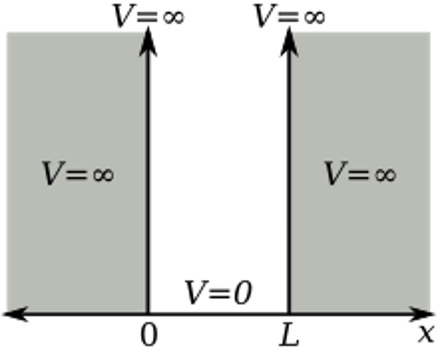
\includegraphics[scale=0.4]{Pot}
\caption{Shéma représentant le potentiel d'une particule dans une boîte}
\end{figure}
\end{columns}
\end{frame}



\section{L'Hamiltonien}
\begin{frame}
\frametitle{Le potentiel}

\begin{columns}
\column{0.6\textwidth}
L'Hamiltonien général pour un système conservatif unidimensionnel est

\begin{equation}\tag{2}
\hat{H}=-\frac{\hbar^2}{2m}\frac{\partial^2}{\partial x^2}+\hat{V}(x)
\end{equation} 

\column{0.4\textwidth}
\begin{figure}
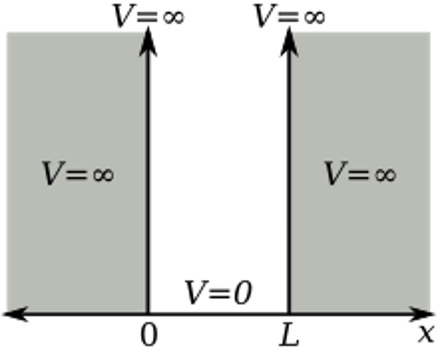
\includegraphics[scale=0.4]{Pot}
\caption{Shéma représentant le potentiel d'une particule dans une boîte}
\end{figure}
\end{columns}

\end{frame}


\section{L'Hamiltonien}
\begin{frame}
\frametitle{Le potentiel}

\begin{columns}
\column{0.6\textwidth}
L'Hamiltonien de ce système est

\begin{equation}\tag{3}
\hat{H}=-\frac{\hbar^2}{2m}\frac{\partial^2}{\partial x^2}
\end{equation} 

\column{0.4\textwidth}
\begin{figure}
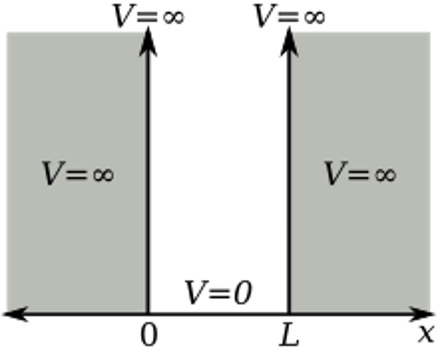
\includegraphics[scale=0.4]{Pot}
\caption{Shéma représentant le potentiel d'une particule dans une boîte}
\end{figure}
\end{columns}

\end{frame}


\section{Équation de Shrödinger indépendante du temps}
\begin{frame}
\frametitle{Équation de Shrödinger indépendante du temps}

\begin{columns}
\column{0.6\textwidth}

\begin{equation}\tag{3}
\hat{H}=-\frac{\hbar^2}{2m}\frac{\partial^2}{\partial x^2}
\end{equation} 

\begin{equation}\tag{4}
\hat{H}\Psi(x)=E\Psi(x)
\end{equation} 

\column{0.4\textwidth}
\begin{figure}
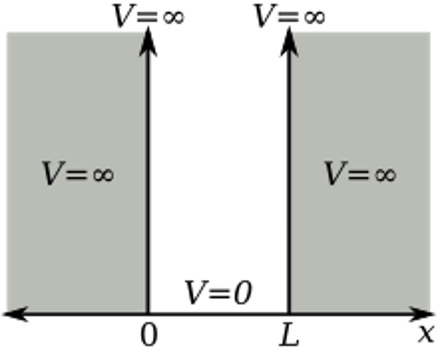
\includegraphics[scale=0.4]{Pot}
\caption{Shéma représentant le potentiel d'une particule dans une boîte}
\end{figure}
\end{columns}

\end{frame}

\begin{frame}
\frametitle{Équation de Shrödinger indépendante du temps}

\begin{columns}
\column{0.6\textwidth}

\begin{equation}\tag{3}
\hat{H}=-\frac{\hbar^2}{2m}\frac{\partial^2}{\partial x^2}
\end{equation} 

\begin{equation}\tag{4}
-\frac{\hbar^2}{2m}\frac{\partial^2}{\partial x^2}\Psi(x)=E\Psi(x)
\end{equation} 

\column{0.4\textwidth}
\begin{figure}
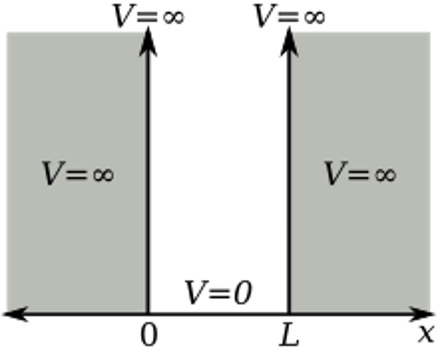
\includegraphics[scale=0.4]{Pot}
\caption{Shéma représentant le potentiel d'une particule dans une boîte}
\end{figure}
\end{columns}

\end{frame}


\begin{frame}
\frametitle{Équation de Shrödinger indépendante du temps}

\begin{columns}
\column{0.6\textwidth}

\begin{equation}\tag{4}
-\frac{\hbar^2}{2m}\frac{\partial^2}{\partial x^2}\Psi(x)=E\Psi(x)
\end{equation} 

\begin{itemize}
\item[]<1-> \begin{equation}\tag{5}
\Psi(x)=A\sin(kx)+B\cos(kx)
\end{equation} 
\item[]<2-> \begin{equation}\tag{6}
\Psi(0)=0
\end{equation} 
\item[]<2-> \begin{equation}\tag{7}
\Psi(L)=0
\end{equation} 
\end{itemize}
\column{0.4\textwidth}
\begin{figure}
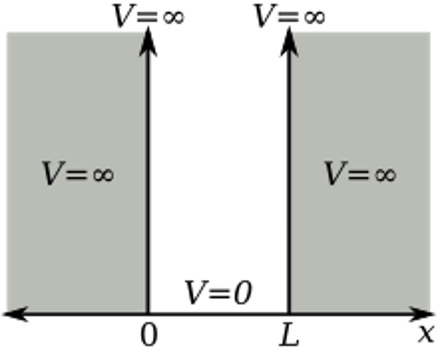
\includegraphics[scale=0.4]{Pot}
\caption{Shéma représentant le potentiel d'une particule dans une boîte}
\end{figure}
\end{columns}

\end{frame}

\begin{frame}
\frametitle{Équation de Shrödinger indépendante du temps}

\begin{columns}
\column{0.6\textwidth}

\begin{equation}\tag{4}
-\frac{\hbar^2}{2m}\frac{\partial^2}{\partial x^2}\Psi(x)=E\Psi(x)
\end{equation} 

\begin{itemize}
\item[]<1-> \begin{equation}\tag{5}
\Psi(x)=A\sin(kx)
\end{equation} 
\item[]<1-> \begin{equation}\tag{6}
B=0
\end{equation} 
\item[]<1-> \begin{equation}\tag{7}
\Psi(L)=0
\end{equation} 
\end{itemize}
\column{0.4\textwidth}
\begin{figure}
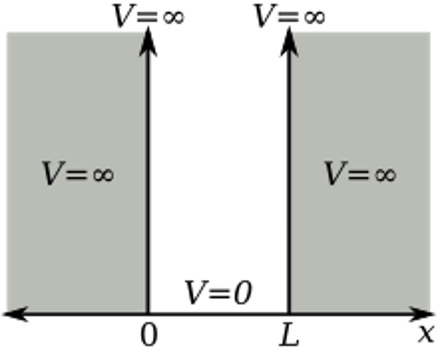
\includegraphics[scale=0.4]{Pot}
\caption{Shéma représentant le potentiel d'une particule dans une boîte}
\end{figure}
\end{columns}

\end{frame}




\begin{frame}
\frametitle{Équation de Shrödinger indépendante du temps}

\begin{columns}
\column{0.6\textwidth}

\begin{equation}\tag{4}
-\frac{\hbar^2}{2m}\frac{\partial^2}{\partial x^2}\Psi(x)=E\Psi(x)
\end{equation} 

\begin{itemize}
\item[]<1-> \begin{equation}\tag{5}
\Psi(x)=A\sin(kx)
\end{equation}  
\item[]<1-> \begin{equation}\tag{6}
\Psi(L)=0
\end{equation}
\item[]<2-> \begin{equation}\tag{7}
\Psi(L)=0=A\sin(kL)
\end{equation} 
\item[]<3-> \begin{equation}\tag{8}
kL=n\pi, n\in \mathbb{N}^*
\end{equation} 
\item[]<4-> \begin{equation}\tag{8}
k=\frac{n\pi}{L}, n\in \mathbb{N}^*
\end{equation} 
\end{itemize}
\column{0.4\textwidth}
\begin{figure}
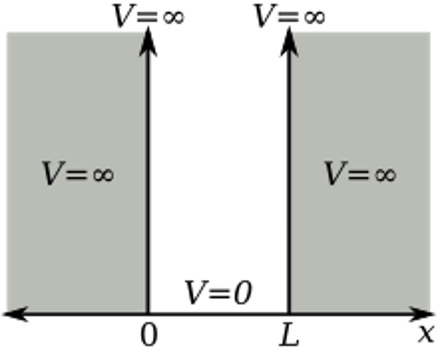
\includegraphics[scale=0.4]{Pot}
\caption{Shéma représentant le potentiel d'une particule dans une boîte}
\end{figure}
\end{columns}

\end{frame}

\begin{frame}
\frametitle{Équation de Shrödinger indépendante du temps}

\begin{columns}
\column{0.6\textwidth}

\begin{equation}\tag{4}
-\frac{\hbar^2}{2m}\frac{\partial^2}{\partial x^2}\Psi_n(x)=E_n\Psi(x)
\end{equation} 

\begin{itemize}
\item[]<1-> \begin{equation}\tag{5}
\Psi_n(x)=A\sin(\frac{n\pi x}{L})
\end{equation}  

\item[]<2-> \begin{equation}\tag{6}
\int dx \Psi_n(x)^* \Psi_n(x)=1
\end{equation}  
\end{itemize}
\column{0.4\textwidth}
\begin{figure}
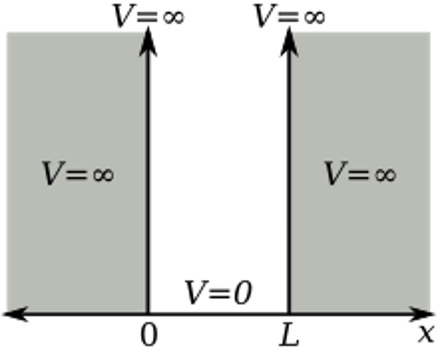
\includegraphics[scale=0.4]{Pot}
\caption{Shéma représentant le potentiel d'une particule dans une boîte}
\end{figure}
\end{columns}

\end{frame}

\begin{frame}
\frametitle{Équation de Shrödinger indépendante du temps}

\begin{columns}
\column{0.6\textwidth}

\begin{equation}\tag{4}
-\frac{\hbar^2}{2m}\frac{\partial^2}{\partial x^2}\Psi_n(x)=E_n\Psi_n(x)
\end{equation} 

\begin{itemize}
\item[]<1-> \begin{equation}\tag{5}
\Psi_n(x)=A\sin(\frac{n\pi x}{L})
\end{equation}  
\item[]<1-> \begin{equation}\tag{6}
\int dx (A\sin(\frac{n\pi x}{L}))(A\sin(\frac{n\pi x}{L}))=1
\end{equation}  
\end{itemize}
\column{0.4\textwidth}
\begin{figure}
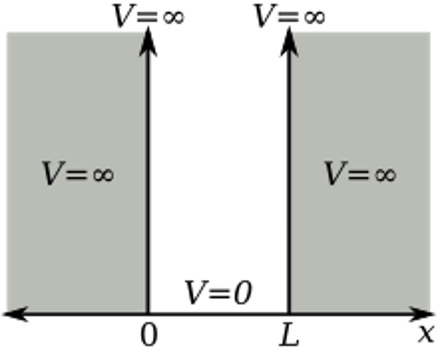
\includegraphics[scale=0.4]{Pot}
\caption{Shéma représentant le potentiel d'une particule dans une boîte}
\end{figure}
\end{columns}

\end{frame}


\begin{frame}
\frametitle{Équation de Shrödinger indépendante du temps}
%
\begin{columns}
\column{0.6\textwidth}
%
\begin{equation}\tag{4}
-\frac{\hbar^2}{2m}\frac{\partial^2}{\partial x^2}\Psi(x)=E\Psi(x)
\end{equation} 
%
\begin{itemize}
\item[]<1-> \begin{equation}\tag{5}
\Psi(x)=A\sin(\frac{n\pi x}{L})
\end{equation}  
\item[]<1-> \begin{equation}\tag{6}
\int dx A^2\sin^2(\frac{n\pi x}{L})=1
\end{equation}
%%\item[]  <2-> \begin{equation}\tag{8}
%%\left. -A^2 2\cos(\frac{n\pi x}{L} )\right|^{L}_{0}=1
%%\end{equation}
\item[]  <2-> \begin{equation}\tag{7}
A^2 \frac{L}{2}=1
\end{equation}
%\end{itemize}
\item[]  <3-> \begin{equation}\tag{7}
A=\sqrt{\frac{2}{L}}
\end{equation}
\end{itemize}
\column{0.4\textwidth}
\begin{figure}
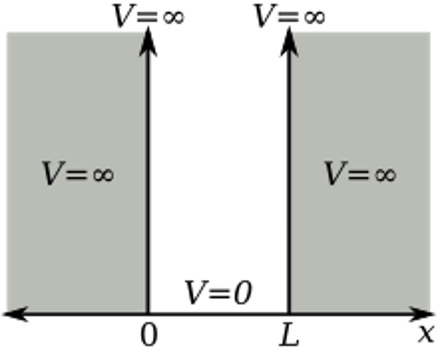
\includegraphics[scale=0.4]{Pot}
\caption{Shéma représentant le potentiel d'une particule dans une boîte}
\end{figure}
\end{columns}
%
\end{frame}

%\begin{frame}
%\frametitle{Équation de Shrödinger indépendante du temps}
%
%\begin{columns}
%\column{0.6\textwidth}
%
%\begin{equation}\tag{4}
%-\frac{\hbar^2}{2m}\frac{\partial^2}{\partial x^2}\Psi_n(x)=E\Psi_n(x)
%\end{equation} 
%
%\begin{itemize}
%\item[]<1-> \begin{equation}\tag{5}
%\Psi_n(x)=A\sin(\frac{n\pi x}{L})
%\end{equation}  
%\item[]<1-> \begin{equation}\tag{6}
%\int dx A^2\sin^2(\frac{n\pi x}{L})=1
%\end{equation}
%%\item[]  <2-> \begin{equation}\tag{8}
%%\left. -A^2 2\cos(\frac{n\pi x}{L} )\right|^{L}_{0}=1
%%\end{equation}
%\item[]  <2-> \begin{equation}\tag{7}
%A=\sqrt{\frac{2}{L}}
%\end{equation}
%\end{itemize}
%\column{0.4\textwidth}
%\begin{figure}
%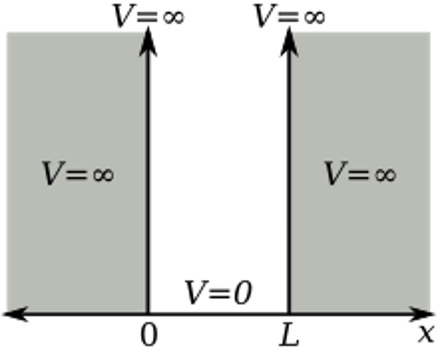
\includegraphics[scale=0.4]{Pot}
%\caption{Shéma représentant le potentiel d'une particule dans une boîte}
%\end{figure}
%\end{columns}
%
%\end{frame}

\begin{frame}
\frametitle{Équation de Shrödinger indépendante du temps}

\begin{columns}
\column{0.6\textwidth}

\begin{equation}\tag{4}
-\frac{\hbar^2}{2m}\frac{\partial^2}{\partial x^2}\Psi_n(x)=E_n\Psi_n(x)
\end{equation} 

\begin{itemize}
\item[]<1-> \begin{equation}\tag{5}
\Psi_n(x)=\sqrt{\frac{2}{L}}\sin(\frac{n\pi x}{L})
\end{equation}  
\item[]<2-> \begin{equation}\tag{6}
-\frac{\hbar^2}{2m}\frac{\partial^2}{\partial x^2}\sqrt{\frac{2}{L}}\sin(\frac{n\pi x}{L})=E_n\Psi_n(x)
\end{equation}  

\item[]<3-> \begin{equation}\tag{7}
\frac{\partial^2}{\partial x^2}\sin(\frac{n\pi x}{L})=-\frac{n^2\pi^2}{L^2}\sin(\frac{n\pi x}{L})
\end{equation} 

\end{itemize}
\column{0.4\textwidth}
\begin{figure}
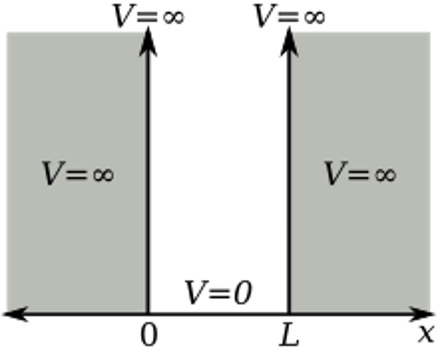
\includegraphics[scale=0.4]{Pot}
\caption{Shéma représentant le potentiel d'une particule dans une boîte}
\end{figure}
\end{columns}

\end{frame}

\begin{frame}
\frametitle{Équation de Shrödinger indépendante du temps}

\begin{columns}
\column{0.6\textwidth}

\begin{equation}\tag{4}
-\frac{\hbar^2}{2m}\frac{\partial^2}{\partial x^2}\Psi_n(x)=E_n\Psi_n(x)
\end{equation} 

\begin{itemize}
\item[]<1-> \begin{equation}\tag{5}
\Psi_n(x)=\sqrt{\frac{2}{L}}\sin(\frac{n\pi x}{L})
\end{equation}  
\item[]<1-> \begin{equation}\tag{6}
\frac{\hbar^2n^2\pi^2}{2mL^2}   \sqrt{\frac{2}{L}}  \sin(\frac{n\pi x}{L})=E_n\Psi_n(x)
\end{equation}  

\item[]<1-> \begin{equation}\tag{7}
\frac{\partial^2}{\partial x^2}\sin(\frac{n\pi x}{L})=-\frac{n^2\pi^2}{L^2}\sin(\frac{n\pi x}{L})
\end{equation} 

\end{itemize}
\column{0.4\textwidth}
\begin{figure}
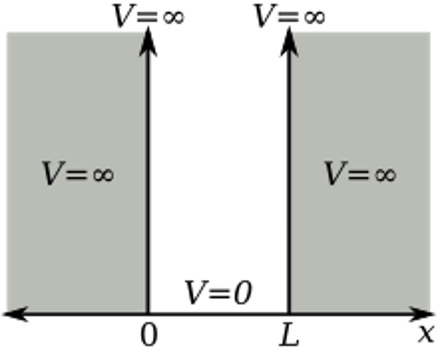
\includegraphics[scale=0.4]{Pot}
\caption{Shéma représentant le potentiel d'une particule dans une boîte}
\end{figure}
\end{columns}

\end{frame}




\begin{frame}
\frametitle{Équation de Shrödinger indépendante du temps}

\begin{columns}
\column{0.6\textwidth}

\begin{equation}\tag{4}
-\frac{\hbar^2}{2m}\frac{\partial^2}{\partial x^2}\Psi_n(x)=E_n\Psi_n(x)
\end{equation} 

\begin{itemize}
\item[]<1-> \begin{equation}\tag{5}
\Psi_n(x)=\sqrt{\frac{2}{L}}\sin(\frac{n\pi x}{L})
\end{equation}  
\item[]<1-> \begin{equation}\tag{6}
\frac{\hbar^2n^2\pi^2}{2mL^2}  \Psi_n(x)=E_n\Psi_n(x)
\end{equation}  

\item[]<1-> \begin{equation}\tag{8}
E_n=\frac{\hbar^2n^2\pi^2}{2mL^2} 
\end{equation} 

\end{itemize}
\column{0.4\textwidth}
\begin{figure}[h]
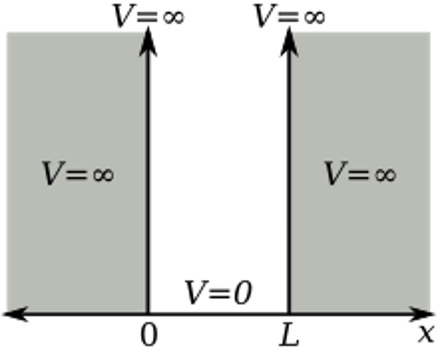
\includegraphics[scale=0.4]{Pot}
\caption{Shéma représentant le potentiel d'une particule dans une boîte}
\end{figure}
\end{columns}

\end{frame}


\begin{frame}
\frametitle{Équation de Shrödinger indépendante du temps}


\begin{equation}\tag{4}
-\frac{\hbar^2}{2m}\frac{\partial^2}{\partial x^2}\Psi_n(x)=E_n\Psi_n(x)
\end{equation} 

\begin{itemize}
\item[]<1-> \begin{equation}\tag{5}
\Psi_n(x)=\sqrt{\frac{2}{L}}\sin(\frac{n\pi x}{L})
\end{equation}  

\item[]<1-> \begin{equation}\tag{8}
E_n=\frac{\hbar^2n^2\pi^2}{2mL^2} 
\end{equation} 
\item[]<1-> \begin{equation}\tag{9}
\hbar=m_e=1 , L=5.0\ u.a. 
\end{equation} 

\end{itemize}

\end{frame}


\begin{frame}
\frametitle{Équation de Shrödinger indépendante du temps}
\begin{figure}[h]
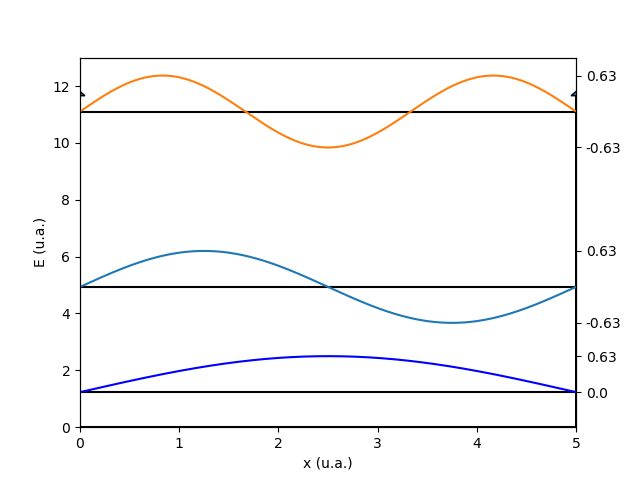
\includegraphics[scale=0.5]{fct_propre}
\caption{Trois première fonctions propres de la particule dans une boîte}
\end{figure}
\end{frame}



\begin{frame}
\frametitle{Équation de Shrödinger indépendante du temps}
\begin{figure}[h]
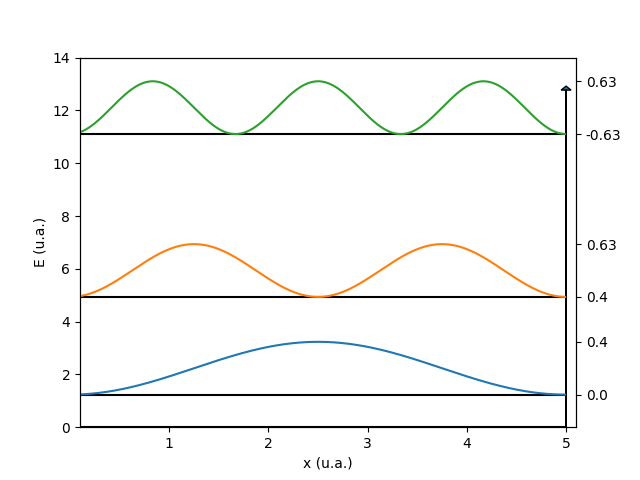
\includegraphics[scale=0.5]{den_propre}
\caption{Trois première fonctions propres de la particule dans une boîte}
\end{figure}

\end{frame}



%---------------------------------------------------------
%Changing visivility of the text
\begin{frame}
\frametitle{Cas 2D}
L'hamiltionien d'une particule libre dans une boîte dimensionnelle est :
\begin{equation}
\hat{H}=-\frac{\hbar^2}{2m}\frac{\partial^2}{\partial x^2}-\frac{\hbar^2}{2m}\frac{\partial^2}{\partial y^2}
\end{equation}
\begin{equation}
\hat{H}=\hat{H}_x+\hat{H}_y
\end{equation}


Pour analyser une particule dans une boîte bidimensionnelle, on peut séparer les variables. 
\begin{equation}
\Psi(x,y)=\psi_x(x)\psi_y(y)
\end{equation}
\end{frame}


\begin{frame}
\frametitle{Cas 2D}
\begin{equation}
\hat{H}\psi_x(x)\psi_y(y)=\hat{H}_x\psi_x(x)\psi_y(y)+\psi_x(x)\hat{H}_y\psi_y(y)
\end{equation}

\begin{equation}
\hat{H}_x\psi_{nx}(x)=E_{nx}\psi_{nx}(x)
\end{equation}
\begin{equation}
\hat{H}_y\psi_{ny}(y)=E_{ny}\psi_{ny}(y)
\end{equation}
\begin{equation}
\hat{H}\Psi_{nx,ny}(x,y)=\left(E_{nx}+E_{ny}\right)\Psi_{nx,ny}(x,y)
\end{equation}
\end{frame}

%---------------------------------------------------------
%Changing visivility of the text
\begin{frame}
\frametitle{Cas 2D}
L'hamiltionien d'une particule libre dans une boîte dimensionnelle est :
\begin{equation}
\hat{H}=-\frac{\hbar^2}{2m}\left(\frac{\partial^2}{\partial x^2}+\frac{\partial^2}{\partial y^2}\right)
\end{equation}

\end{frame}


\begin{frame}
\frametitle{Cas 2D}
\begin{equation}
\hat{H}\psi_x(x)\psi_y(y)=-\frac{\hbar^2}{2m}\left(\frac{\partial^2}{\partial x^2}\psi_x(x)\psi_y(y)+\psi_x(x)\frac{\partial^2}{\partial y^2}\psi_y(y)\right)
\end{equation}

Pour analyser une particule dans une boîte bidimensionnelle, on peut séparer les variables. 
\begin{equation}
\Psi(x,y)=\psi_x(x)\psi_y(y)
\end{equation}
\end{frame}




\begin{frame}
\frametitle{Équation de Shrödinger indépendante du temps}
\begin{figure}[h]
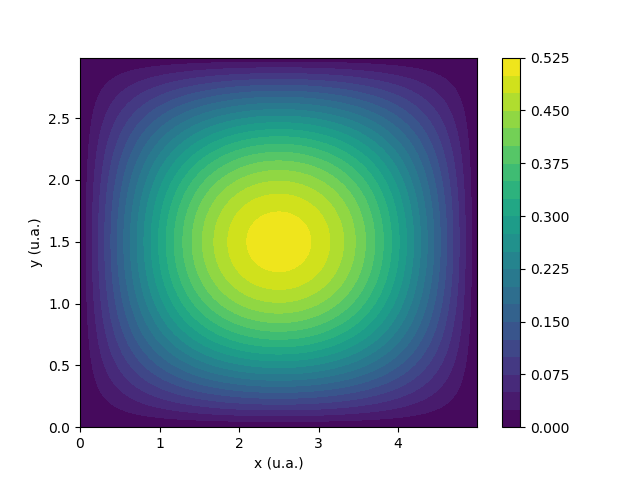
\includegraphics[scale=0.5]{fct_propre2d_11}
\caption{Fonction propre $\psi_{1,1}(x,y)$ d'une boîte bidimensionnelle de dimension $L_x=5\ u.a.$ et $L_y=3\ u.a.$}
\end{figure}
\end{frame}


\begin{frame}
\frametitle{Équation de Shrödinger indépendante du temps}
\begin{figure}[h]
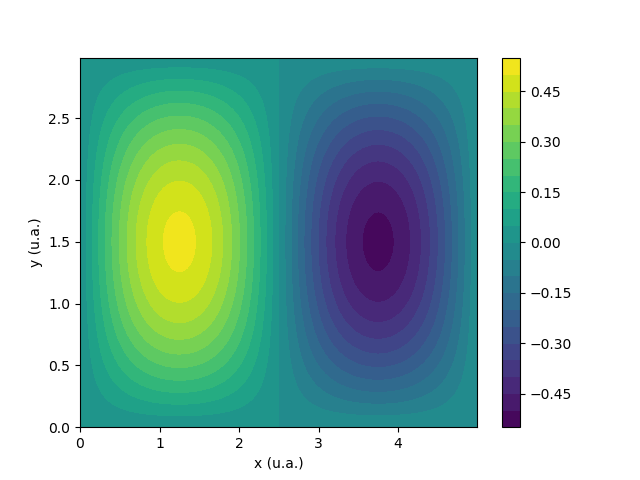
\includegraphics[scale=0.5]{fct_propre2d_21}
\caption{Fonction propre $\psi_{2,1}(x,y)$ d'une boîte bidimensionnelle de dimension $L_x=5\ u.a.$ et $L_y=3\ u.a.$}
\end{figure}
\end{frame}


\begin{frame}
\frametitle{Équation de Shrödinger indépendante du temps}
\begin{figure}[h]
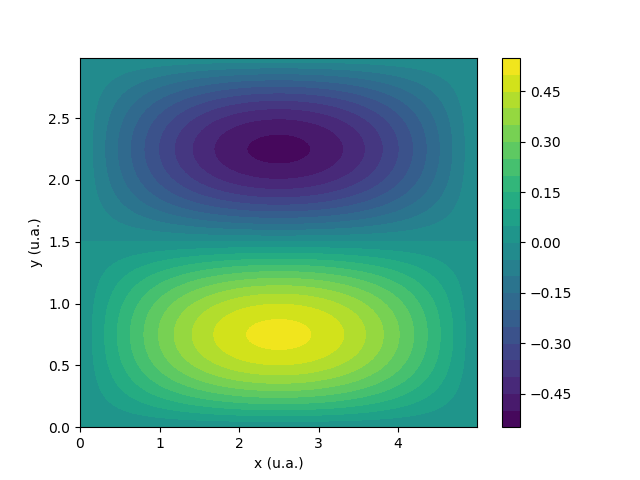
\includegraphics[scale=0.5]{fct_propre2d_12}
\caption{Fonction propre $\psi_{1,2}(x,y)$ d'une boîte bidimensionnelle de dimension $L_x=5\ u.a.$ et $L_y=3\ u.a.$}
\end{figure}
\end{frame}


\begin{frame}
\frametitle{Équation de Shrödinger indépendante du temps}
\begin{figure}[h]
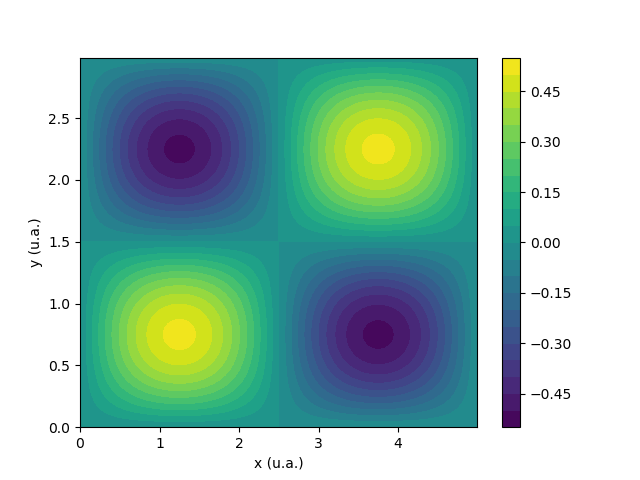
\includegraphics[scale=0.5]{fct_propre2d_22}
\caption{Fonction propre $\psi_{2,2}(x,y)$ d'une boîte bidimensionnelle de dimension $L_x=5\ u.a.$ et $L_y=3\ u.a.$}
\end{figure}
\end{frame}


\end{document}



